\subsection{Обзор существующих аналогов}
\label{sec:analysis:analogues}

Для решения задач управления процессом проведения викторин и их создания могут использоваться различные средства. Рассмотрим каждую из задач в отдельности.

\subsubsection{} Управление процессом создания викторин
\label{sec:analysis:analogues:create_quest}

Для организаторов проведения викторин важнейшим аспектом является необмходимость в предварительно составленных викторинах по желаемой тематике.
Человеку известно тысячи различным областей знаний по самым разным предметам изучения и необходимо иметь возможность создать викторину по любой тематике, которая только может
придти в голову, причем для повышения уровня вовлеченности в игровой процесс следует использовать нечто большее, чем просто текст.

Одним из безусловных лидеров в области проведения викторин является программное средство SIGame, разработанное Владимиром Хилем. Для проведения викторин их необходимо предварительно 
создать в программном средстве, поставляемым отдельно под названием SIQuester. Данное программное средство позволяет создавать пакеты вопросов для дальнейшего использования
в SIGame. Интерфейс приложения выглядит как изображено на рисунке \ref*{sec:analysis:analogues:create_quest:siquester}.

\begin{figure}[!ht]
	\centering
	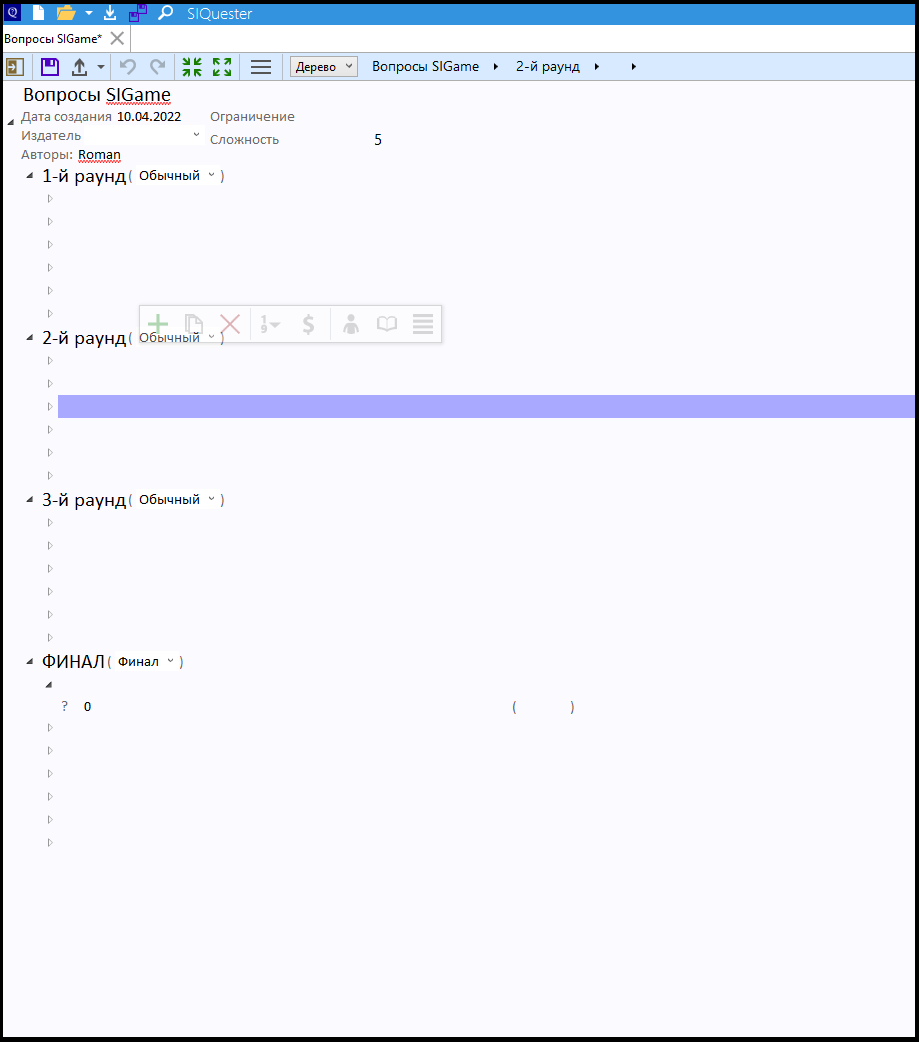
\includegraphics[scale=0.65]{attachments/siquester.png}  
	\caption{Интерфейс приложения SIQuester}
	\label{sec:analysis:analogues:create_quest:siquester}
\end{figure}

SIQuester поддерживает создание различных видов вопросов, как по содержанию, так и по формату разыгровки, среди поддерживаемых вопросов по содержанию есть:

\begin{itemize}
	\item текст;
	\item изображение;
	\item фрагмент видео;
	\item звуковой фрагмент.
\end{itemize} 

По формату разыгровки вопросов поддерживаются следующие варианты:

Простой вопрос -- отвечающий получает баллы в случае правильного ответа и теряет их в случае неверного ответа, это наболее частовстречающийся вопрос.

Вопрос со ставкой -- перед тем как игроки узнают содержимое вопроса происходит аукцион за право отвечать на вопрос. Тот, кто поставит больше очков и получить право отвечать на вопрос
при этом награда за правильный ответ или штраф за неправильный будет является финальным размером ставки на аукционе.

Вопрос с секретом -- тема вопроса, а также его стоимость может не совпадать с той, которая указана в сетке вопросов. В этом и заключается секретность вопроса. Этот вопрос также 
можно передать любому из участников.

Вопрос без риска -- в случае неправильного ответа участник, отвечающий на вопрос не теряет баллы, равные стоимости вопроса.

Примеры вопросов разных типов приведены на рисунке \ref*{sec:analysis:analogues:create_quest:siquester_types}.

\begin{figure}[!ht]
	\centering
	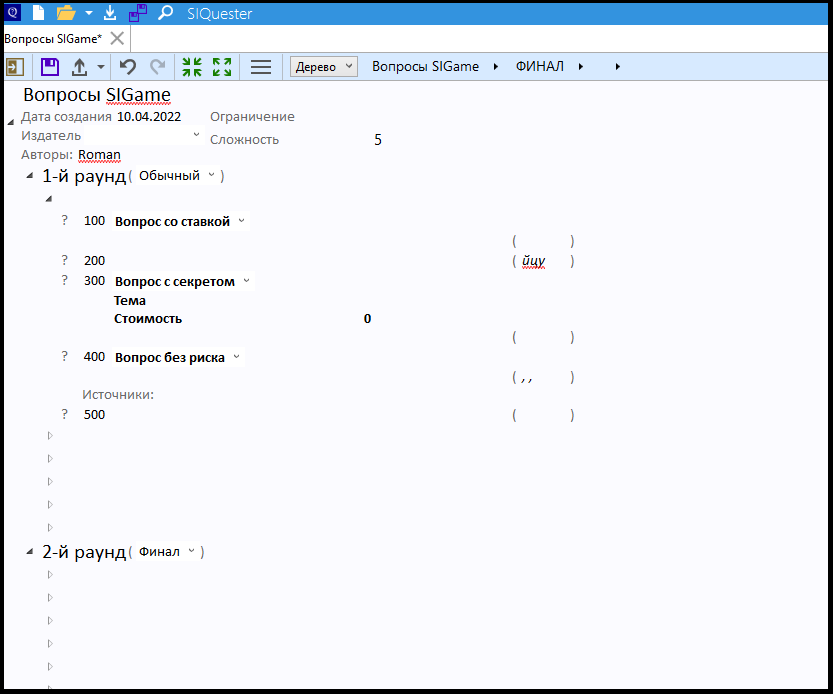
\includegraphics[scale=0.6]{attachments/siquester_types.png}  
	\caption{Примеры вопросов в SIQuester}
	\label{sec:analysis:analogues:create_quest:siquester_types}
\end{figure}

Анализ существующих аналогов по созданию вопросов показывает возможность наличия различных интерактивных видов вопросов для повышения заинтересованности игроков 
в игровом процессе и повышения уровня эмоционального удовлетворения в результате игры, но в то же время такой подход усложняет игровой процесс для совсем неопытных игроков,
поэтому в данном курсовом проекте будет использоваться единственный тип вопроса -- простой.

\subsubsection{} Управление процессом идентификации игроков
\label{sec:analysis:analogues:create_acc}

Для идентификации в сети в программном средстве используется анонимный подход: не нужны никакие средства внешней идентификации пользователя, такие как электронная почта,
номер телефона и так далее. Экран создания локального аккаунта для игры выглядит следующим образом (рисунок \ref{sec:analysis:analogues:create_acc:sigame_acc})

\begin{figure}[!ht]
	\centering
	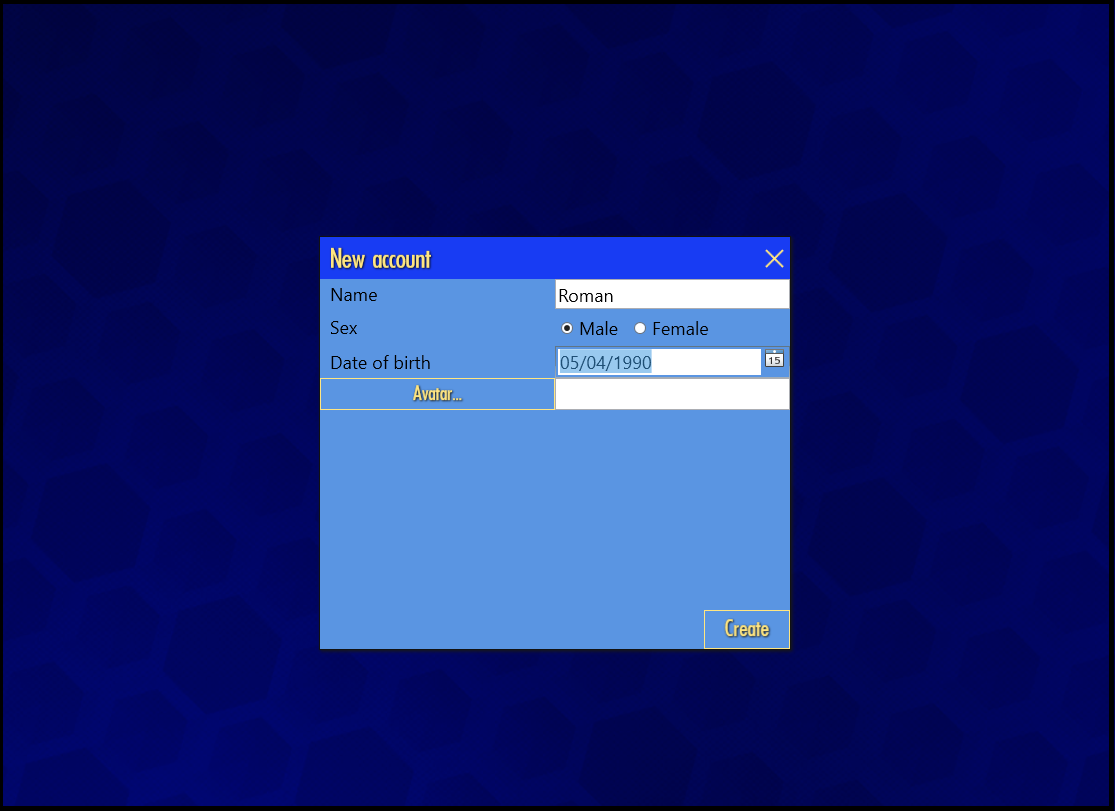
\includegraphics[scale=0.5]{attachments/sigame_acc.png}  
	\caption{Создание аккаунта в SIGame}
	\label{sec:analysis:analogues:create_acc:sigame_acc}
\end{figure}

Из этого можно сделать вывод, что аккаунты носят минимально функциональный характер и служит средством идентификации для
людей, которые и так уже знают игроков в реальной жизни, поэтому злоумышленник не сможет украсть какие-либо конфиденциальные данные,
так как приложение их нигде не хранит и не использует, а для проведения викторин они не требуются. 

Анализ показывает, что аккаунты в такого рода программных средствах используются лишь из необходимости минимальной идентификации в процессе игры и не служат для
сбора информации, поэтому смысла реализовывать какого либо рода защиту нет.

\subsubsection{} Управление процессом создания игры
\label{sec:analysis:analogues:host_game}

Перед тем как игроки смогут подключится к игре, необходимо, чтобы ведущий создал игровое лобби, пример реализации процесса создания лобби в SIGame изображен на 
рисунке \ref{sec:analysis:analogues:host_game:sigame_host}. 

\begin{figure}[!ht]
	\centering
	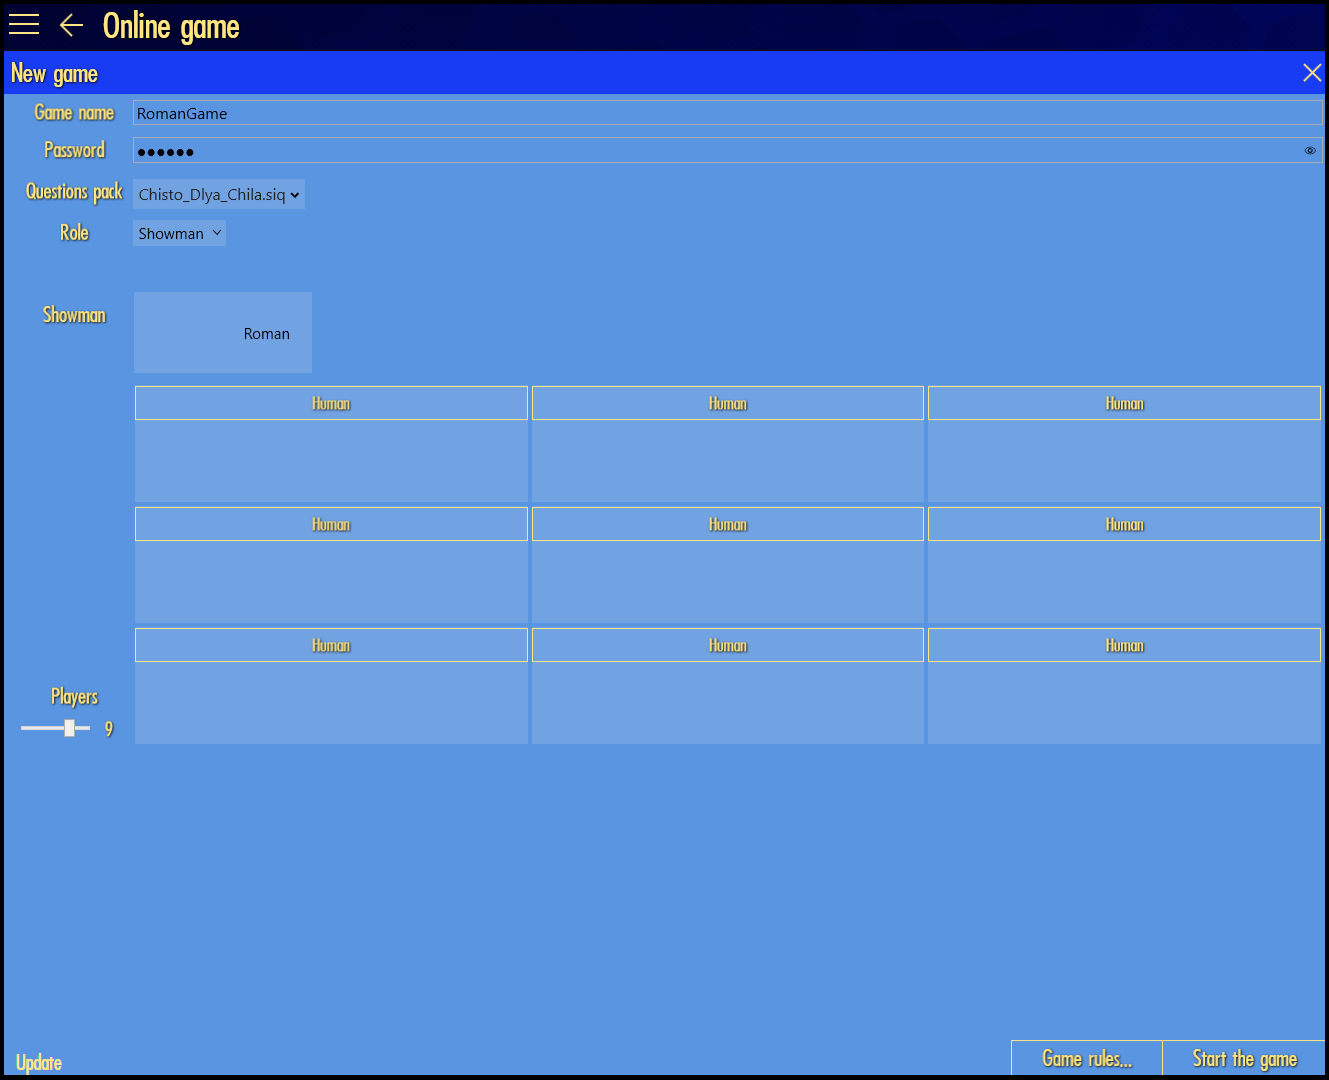
\includegraphics[scale=0.4]{attachments/sigame_host.png}  
	\caption{Создание игрового лобби в SIGame}
	\label{sec:analysis:analogues:host_game:sigame_host}
\end{figure}

Настройка лобби отвечает за несколько важных особенностей проведения викторины.

Название лобби позволяет игрокам, желающим присоединится к состязанию, найти игру в списке всех доступных игр, а зная название сделать это намного проще.

Пароль позволяет хосту защитить лобби от ограничить доступ нежелательным игрокам и оставить лишь тем, кто знает пароль.

Настройка вопросов позволяет выбрать заранее созданный в програм-ме тестере набор вопросов, на которые предстоит отвечать игрокам.

Размер игрового лобби позволяет устанавливать лимит на максимальное количество активных игроков в сессии, что позволит избежать слишком большого количества игроков в случае
создания игры без пароля.

Анализ показывает, что создание лобби это обязательная часть программного средства и от ее реализации зависит игровой опыт, который получат игроки в процессе проведения викторины.
Минимальный набор настроек, необходимых для настройки лобби были перечислены выше и требуются для дальнейшей реализации игрового процесса.

\subsubsection{} Управление процессом подключения к игре
\label{sec:analysis:analogues:join_game}

Игроки используют процесс подключения к игре, для того, чтобы попасть в одно игровое лобби с организатором викторины.
Процесс подключения к игровому лобби выглядит следующим образом (рисунок \ref{sec:analysis:analogues:join_game:sigame_join}).

\begin{figure}[!ht]
	\centering
	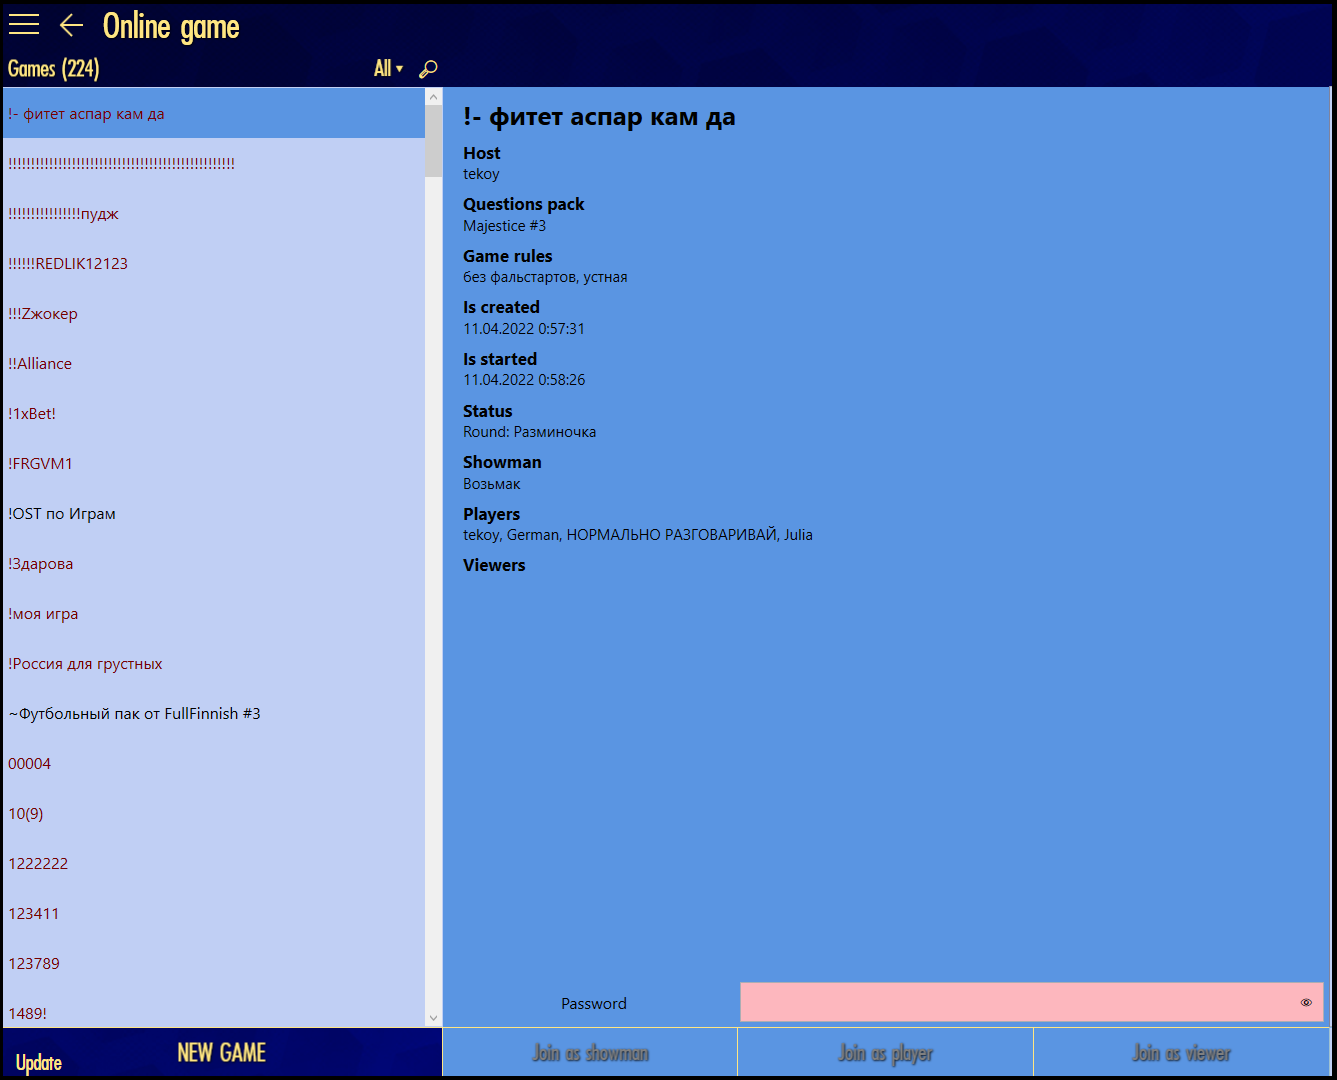
\includegraphics[scale=0.4]{attachments/sigame_join.png}  
	\caption{Подключение к игровому лобби в SIGame}
	\label{sec:analysis:analogues:join_game:sigame_join}
\end{figure}

Перед пользователем представлен список доступных игр для подключения, которые можно идентифицировать по названию игрового лобби и его организатору.
В случае, если лобби имеет пароль, то при подключении появляется модальное окно, где его необходимо ввести. После подключения пользователь попадает в лобби и 
может приступать к игровому процессу.

Анализ показывает, что процесс подключения к игре является одним из важнейших во всем программном средстве. Без возможности подключится к игровому лобби смысл
программного средства теряется.

\subsubsection{} Управление игровым процессом
\label{sec:analysis:analogues:game}

Игровой процесс заключается в поочередном ответе на вопросы и зачислении очков, победителем считается тот, кто набрал больше всего очков к моменту, когда закончатся все вопросы.
Фрагмент игрового процесса представлен на рисунке \ref{sec:analysis:analogues:game:sigame_game}.

\begin{figure}[!ht]
	\centering
	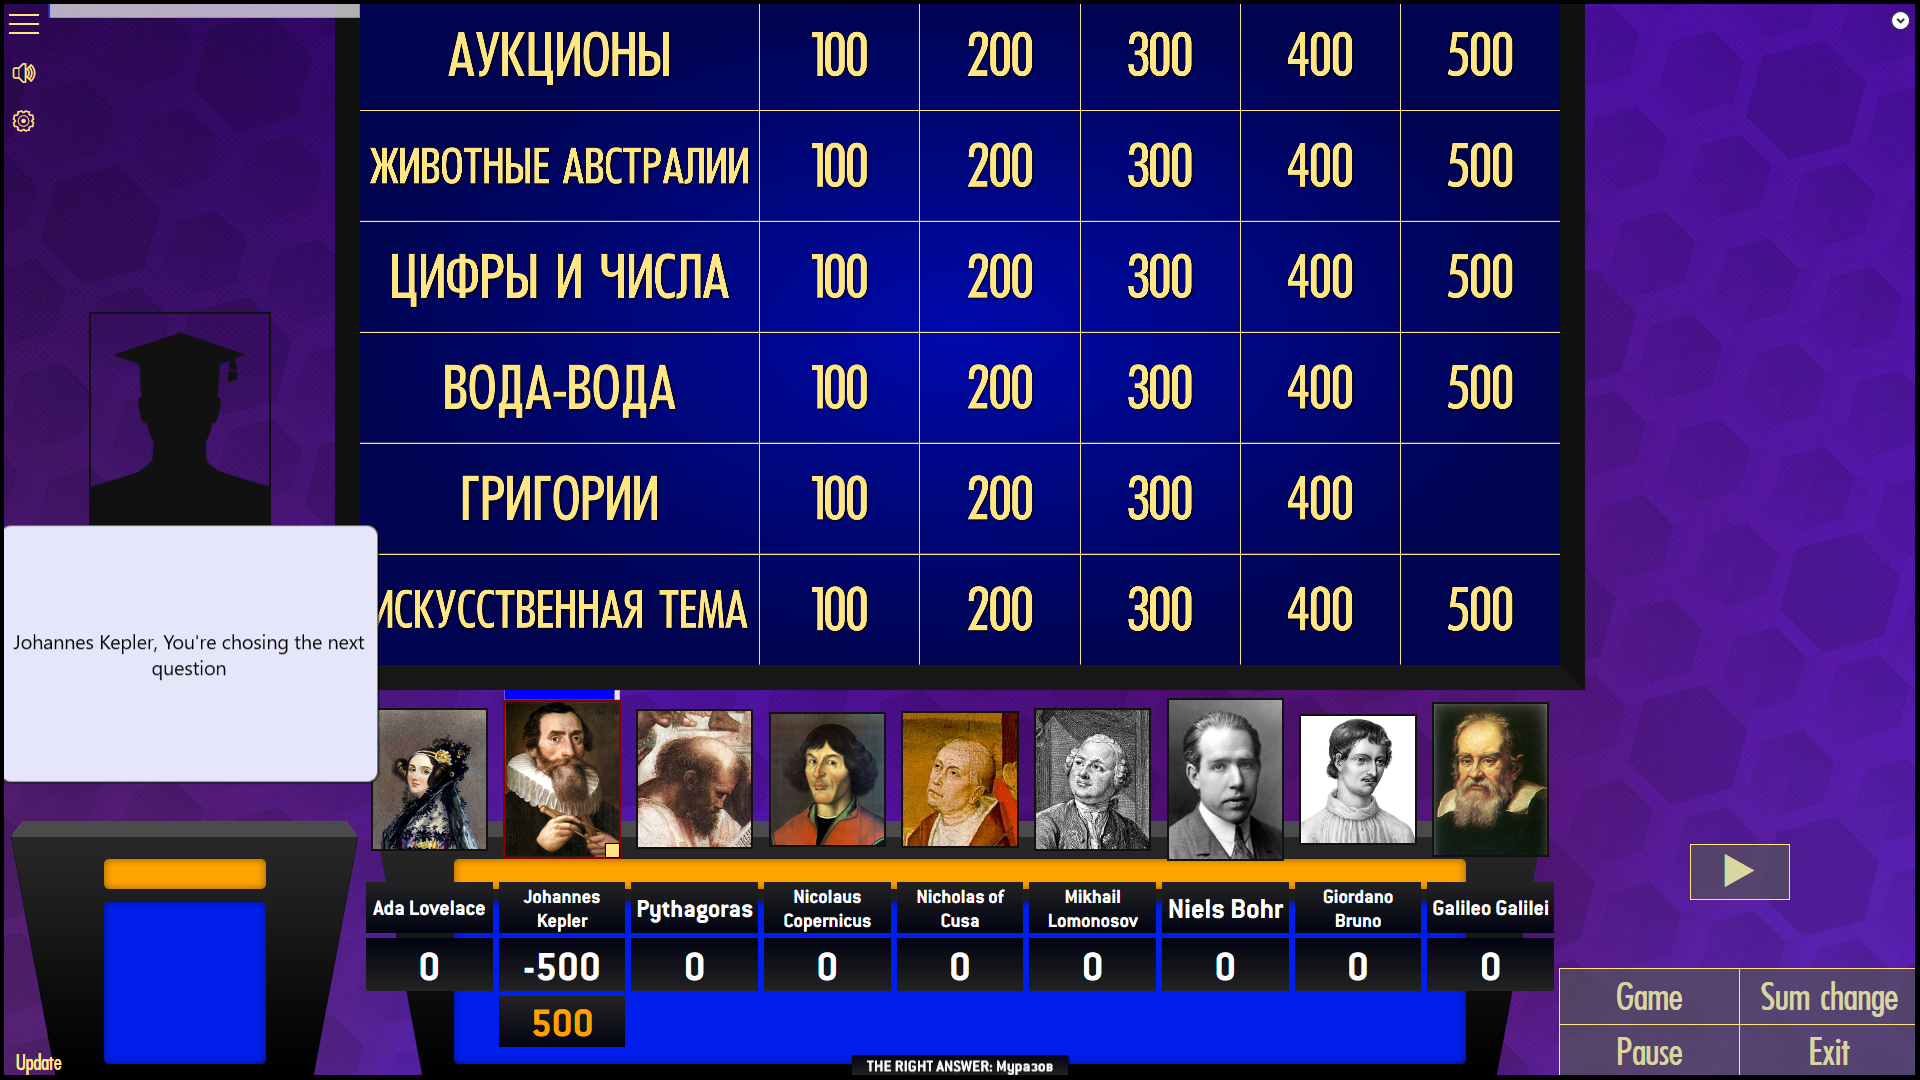
\includegraphics[scale=0.30]{attachments/sigame_game.png}  
	\caption{Процесс игры в SIGame}
	\label{sec:analysis:analogues:game:sigame_game}
\end{figure}

Следует отметить, что хотя сам игровой процесс является довольно простым, при этом он также является достаточно увлекательным, чтобы на долго время задерживать игроков и оставаться
увлеченным. Игроки отвечают на вопросы, в то время как ведущий контролирует правильность ответов и решает начислять очки, или нет. Здесь следует сделать оговорку, что предполагается,
что игра проходит в устной форме, т. е. игроки общаются между собой посредством внешнего программного средства для голосовой связи, например: Discord, Skype и так далее, поэтому реализация
средств коммуникации непосредственно в приложении не является необходимой.

Анализ показывает, что наибольшее внимание стоит уделить релизации логики игрового процесса, так как от него напрямую зависит удовлетворенность игроков процессом проведения викторин.

\subsubsection{} Обзор иных программных средств для проведения викторин
\label{sec:analysis:analogues:other_programs}

Рассмотренные процессы типичны для любого приложения с ориентацией на взаимодействие по сети, в то время как проведение викторин имеет свои особенности в разных реализациях.

Веб-аналоги позволяют избежать установки на персональный компьютер, но в то же время увеличивают нагрузку на сеть, что может быть не приемлемо для некоторых категорий пользователей.
К тому же в случае ограничения доступа к сайту или отказа в обслуживании больше воспользоваться программным средством не получится.

Реализации для мобильных телефонов имеют более скромный функционал по сравнению с версией для настольного компьютера, это обусловлено тем, что небольшой экран и нестабильное интернет-соединение
не могут обеспечить достаточный уровень комфорта при игре. К тому же общение с игроками затруднено тем, что использование средств связи на мобильном телефоне параллельно с проведением викторины
не является удобным, поэтому популярность такие реализации не снискали.

После анализа типичных реализаций был сделан вывод, что наилучшим решением для разработки программного средства проведения многопользовательских викторин является настольное приложение.
